% !TEX root = hazel-LIVE2018.tex

\section{Live Palettes}
\label{sec:palettes}


\begin{figure}[t]
\vspace{-4px}
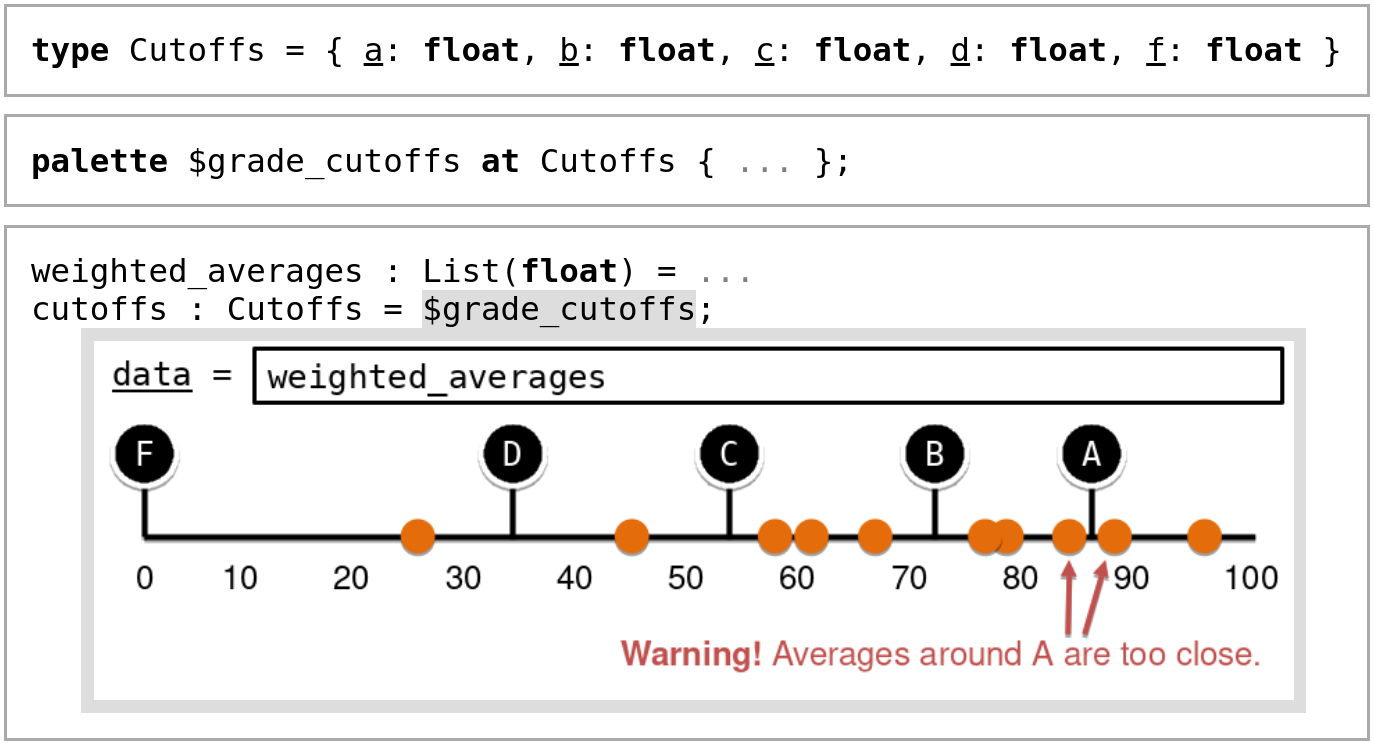
\includegraphics[width=0.7\textwidth]{images/cutoffs-new-elided.png}
\caption{An example where the teacher assigns cutoffs 
for letter grades using a domain-specific live palette.}
\label{fig:cutoffs-example}
\vspace{-7px}
\end{figure}

Another editor service that we are designing for integration into \Hazel 
is the \emph{live palette} service.
Palettes, which were introduced in work on
\emph{active code completion} by \citet{ActiveCodeCompletion},  allow programmers to fill typed 
holes by directly manipulating specialized graphical user interfaces rather than by exclusively entering symbolic
code. For example, a palette might allow the programmer to 
fill in a hole of type \li{Color} using a color selection  
user interface, rather than by construcing a \li{Color} value  
by manually typing the necessary code. \citet{ActiveCodeCompletion} elicited a large number of other
examples of data types where an alternative, graphical 
method of constructing a value of a particular type might be
useful. Due to the large number of examples, the system in that paper, called {Graphite}, is designed to be extensible by library providers. 

Palettes in {Graphite} 
are ephemeral, operating as a form of code completion, but projectional editors, e.g. Barista \cite{ko_barista:_2006} and \li{mbeddr} \cite{voelter_mbeddr:_2012}, often support a small fixed number of  
palettes (there called \emph{projections}) that persist, i.e. that appear within the code itself. 
Projectional palettes also improve upon Graphite's palettes in that they are compositional, i.e. they allow code to appear within holes that appear inside the palette (e.g. the entries in a matrix palette). 

Like Graphite, \Hazel's palette system (which is currently in the design phase) is extensible. 
Like projectional palettes, \Hazel's palettes are also persistent and compositional. 
Holes that appear inside palettes
are governed by a hygiene discipline based on recent work on splicing in user-defined literal macros
\cite{tlms-icfp18}. 
Uniquely, \Hazel's palette system is live: the program 
can be evaluated before the palette has generated code
and the palette can use the hole closures associated with the hole that it is filling 
to provide concrete feedback to the programmer within the UI.

Let us consider an illustrative domain-specific example that demonstrates
all of these qualities: 
Fig.~\ref{fig:cutoffs-example} shows a mockup of a palette that allows the teacher to determine grade cutoffs, represented collectively by a value of the type \li{Cutoffs} defined in the first cell, by dragging markers visually along a number line, with the student's grades superimposed. The grades are provided by filling a hole in the UI (in this case with \li{weighted_averages}, elided). 
The program is initially evaluated as if the hole where the palette name appears, here \li{$grade_cutoffs}, is empty so that 
any hole closures in the result can be made available to the palette. In this case, there is only one hole closure, from which the
actual value of the variable \li{weighted_averages} can be 
used by the palette to display the grades as orange points.
It can also use this information in other ways, e.g. to point
out that the ``A'' cutoff does not have a very large gap around
it. If there were multiple closures available, the user could
toggle between them using the live palette inspector as discussed in the previous section.

%
The implementation of \li{$grade_cutoffs}, in the second cell, is elided, but each palette is required to implement a
Model-Update-View interface, following the Elm architecture \cite{ElmArchitecture}. 
In the \li{view} function that generates the user
interface as a value of type \li{Html}, the palette may request that a nested hole be
rendered using the \li{HtmlHole} constructor of the \li{Html} type, providing an expected type. When the cursor is in this hole, \Hazel provides all of the usual editor services based on the specified type. Values of the expressions in these holes 
can be requested, relative to the current user-selected closure, for use by the \li{view} function (here, to generate the orange dots as just described). 
Each palette must
also implement a \li{to_exp} function that produces the final
hole filling, much like a macro (see \cite{tlms-icfp18}).
%% for it (\li{hole\_spec.id}) and specifying its type
%% (\li{hole\_spec.type}).
